\documentclass[a4paper,11pt,twoside,draft=false]{scrbook}

\usepackage{UniWien_MSc-Deckblatt}

\usepackage{graphicx}
\usepackage{subcaption}
\usepackage[shortlabels]{enumitem}
\usepackage{amssymb}
\usepackage{amsthm}
\usepackage{amsmath}
\usepackage{mathtools}
\usepackage{braket}
\usepackage{bbm}
\usepackage{graphicx}
\usepackage{float}
\usepackage{scratch}
\usepackage{algorithm}
\usepackage{algpseudocode}
\usepackage[colorlinks=true,naturalnames=true,plainpages=false,pdfpagelabels=true]{hyperref}

\usepackage{tikz}
\usetikzlibrary{patterns,decorations.pathmorphing,positioning}
\usetikzlibrary{calc,decorations.markings, shapes.geometric}
\usepackage[framemethod=TikZ]{mdframed}
\tikzstyle{titlered} =
    [draw=black, thick, fill=white,%
        text=black, rectangle,
        right, minimum height=.7cm]

\usepackage[backend=biber, sorting=none]{biblatex}
\addbibresource{./cite.bib}

\newcommand{\eps}{\varepsilon}
\DeclareMathOperator*{\argmax}{arg\,max}
\DeclareMathOperator*{\argmin}{arg\,min}
\renewcommand{\algorithmicrequire}{\textbf{Input:}}
\renewcommand{\algorithmicensure}{\textbf{Output:}}
% Node styles
\tikzstyle{new style 0}=[fill={rgb,255: red,128; green,128; blue,128},
draw=black, shape=circle, inner sep=0.5mm]
\tikzstyle{1}=[fill=white, draw=black, shape=circle, font=\scriptsize,
        inner sep=0.5mm, outer sep=0.5mm, minimum width=0.5mm]
% Edge styles
\tikzstyle{new edge style 0}=[-, draw={rgb,255: red,191; green,191; blue,191}, ultra thin]
\tikzstyle{new edge style 1}=[-, draw={rgb,255: red,191; green,0; blue,64},
ultra thick]
\tikzstyle{new edge style 2}=[-, draw={rgb,255: red,191; green,0; blue,64}, in=60, out=120, dotted]

\usepackage[most]{tcolorbox}
\tcbuselibrary{skins,breakable}
\colorlet{colexam}{black}
\numberwithin{equation}{subsection}

\newcounter{definition}
\newtcolorbox[use counter=definition, number within=subsection]{definition}[1][]{
    empty,
    title={\textbf{Definition~\thetcbcounter} \textit{#1}},
    attach boxed title to top left,
    boxed title style={
        empty,
        size=minimal,
        bottomrule=1pt,
        top=1pt,
        left skip=0cm,
        overlay=
            {\draw[colexam,line width=1pt]([yshift=-0.35cm]frame.north
        west)--([yshift=-0.35cm]frame.north east);}},
            coltitle=colexam,
            fonttitle=\normalfont,
            before=\par\medskip\noindent,
            parbox=false,
            boxsep=-1pt,
            left=0.75cm,
            right=3mm,
            top=4pt,
            breakable,
            pad at break*=0mm,
            vfill before first,
            overlay unbroken={
                \draw[colexam,line width=1pt]
                ([xshift=0.6cm, yshift=-0.5pt]frame.south
                west)--([xshift=0.6cm,yshift=-1pt]frame.north west)
                --([xshift=0.6cm]frame.south west)--([xshift=-13cm]frame.south east); },
            overlay first={
                \draw[colexam,line width=1pt]
                ([xshift=0.6cm, yshift=-0.5pt]frame.south
                west)--([xshift=0.6cm,yshift=-1pt]frame.north west)
                --([xshift=0.6cm]frame.south west); },
            overlay last={
                \draw[colexam,line width=1pt]
                ([xshift=0.6cm, yshift=-0.5pt]frame.south
                west)--([xshift=0.6cm,yshift=-1pt]frame.north west)
                --([xshift=0.6cm]frame.south west)--([xshift=-13cm]frame.south east); }
}

\newcounter{theorem}
\newtcolorbox[use counter=theorem, number within=subsection]{theorem}[1][]{
    empty,
    title={\textbf{Theorem~\thetcbcounter} \textit{#1}},
    attach boxed title to top left,
    boxed title style={
        empty,
        size=minimal,
        bottomrule=1pt,
        top=1pt,
        left skip=0cm,
        overlay=
            {\draw[colexam,line width=1pt]([yshift=-0.35cm]frame.north
        west)--([yshift=-0.35cm]frame.north east);}},
            coltitle=colexam,
            fonttitle=\normalfont,
            before=\par\medskip\noindent,
            parbox=false,
            boxsep=-1pt,
            left=0.75cm,
            right=3mm,
            top=4pt,
            breakable,
            pad at break*=0mm,
            vfill before first,
            overlay unbroken={
                \draw[colexam,line width=1pt]
                ([xshift=0.6cm, yshift=-0.5pt]frame.south
                west)--([xshift=0.6cm,yshift=-1pt]frame.north west)
                --([xshift=0.6cm]frame.south west)--([xshift=-13cm]frame.south east); },
            overlay first={
                \draw[colexam,line width=1pt]
                ([xshift=0.6cm, yshift=-0.5pt]frame.south
                west)--([xshift=0.6cm,yshift=-1pt]frame.north west)
                --([xshift=0.6cm]frame.south west); },
            overlay last={
                \draw[colexam,line width=1pt]
                ([xshift=0.6cm, yshift=-0.5pt]frame.south
                west)--([xshift=0.6cm,yshift=-1pt]frame.north west)
                --([xshift=0.6cm]frame.south west)--([xshift=-13cm]frame.south east); }
}
\newcounter{lemma}
\newtcolorbox[use counter=lemma, number within=subsection]{lemma}{
    empty,
    title={Lemma~\thetcbcounter},
    attach boxed title to top left,
    boxed title style={
        empty,
        size=minimal,
        bottomrule=1pt,
        top=1pt,
        left skip=0cm,
        overlay=
            {\draw[colexam,line width=1pt]([yshift=-0.35cm]frame.north
        west)--([yshift=-0.35cm]frame.north east);}},
            coltitle=colexam,
            fonttitle=\bfseries,
            before=\par\medskip\noindent,
            parbox=false,
            boxsep=-1pt,
            left=0.75cm,
            right=3mm,
            top=4pt,
            breakable,
            pad at break*=0mm,
            vfill before first,
            overlay unbroken={
                \draw[colexam,line width=1pt]
                ([xshift=0.6cm, yshift=-0.5pt]frame.south
                west)--([xshift=0.6cm,yshift=-1pt]frame.north west)
                --([xshift=0.6cm]frame.south west)--([xshift=-13cm]frame.south east); },
            overlay first={
                \draw[colexam,line width=1pt]
                ([xshift=0.6cm, yshift=-0.5pt]frame.south
                west)--([xshift=0.6cm,yshift=-1pt]frame.north west)
                --([xshift=0.6cm]frame.south west); },
            overlay last={
                \draw[colexam,line width=1pt]
                ([xshift=0.6cm, yshift=-0.5pt]frame.south
                west)--([xshift=0.6cm,yshift=-1pt]frame.north west)
                --([xshift=0.6cm]frame.south west)--([xshift=-13cm]frame.south east); }
}
\newcounter{proposition}
\newtcolorbox[use counter=proposition, number within=subsection]{proposition}{
    empty,
    title={\textbf{Proposition~\thetcbcounter}},
    attach boxed title to top left,
    boxed title style={
        empty,
        size=minimal,
        bottomrule=1pt,
        top=1pt,
        left skip=0cm,
        overlay=
            {\draw[colexam,line width=1pt]([yshift=-0.4cm]frame.north
        west)--([yshift=-0.4cm]frame.north east);}},
            coltitle=colexam,
            fonttitle=\normalfont,
            before=\par\medskip\noindent,
            parbox=false,
            boxsep=-1pt,
            left=0.75cm,
            right=3mm,
            top=4pt,
            breakable,
            pad at break*=0mm,
            vfill before first,
            overlay unbroken={
                \draw[colexam,line width=1pt]
                ([xshift=0.6cm, yshift=-0.5pt]frame.south
                west)--([xshift=0.6cm,yshift=-1pt]frame.north west)
                --([xshift=0.6cm]frame.south west)--([xshift=-13cm]frame.south east); },
            overlay first={
                \draw[colexam,line width=1pt]
                ([xshift=0.6cm, yshift=-0.5pt]frame.south
                west)--([xshift=0.6cm,yshift=-1pt]frame.north west)
                --([xshift=0.6cm]frame.south west); },
            overlay last={
                \draw[colexam,line width=1pt]
                ([xshift=0.6cm, yshift=-0.5pt]frame.south
                west)--([xshift=0.6cm,yshift=-1pt]frame.north west)
                --([xshift=0.6cm]frame.south west)--([xshift=-13cm]frame.south east); }
}
\newcounter{myproof}
\newtcolorbox[]{myproof}[1]{
    empty,
    title={\textbf{Proof}~\textit{#1}},
    attach boxed title to top left,
    boxed title style={
        empty,
        size=minimal,
        bottomrule=1pt,
        top=1pt,
        left skip=0cm,
        overlay=
            {\draw[colexam,line width=1pt]([yshift=-0.35cm]frame.north
        west)--([yshift=-0.35cm]frame.north east);}},
            coltitle=colexam,
            fonttitle=\normalfont,
            before=\par\medskip\noindent,
            parbox=false,
            boxsep=-1pt,
            left=0.75cm,
            right=3mm,
            top=4pt,
            breakable,
            pad at break*=0mm,
            vfill before first,
            overlay unbroken={
                \draw[colexam,line width=1pt]
                ([xshift=0.6cm, yshift=-0.5pt]frame.south
                west)--([xshift=0.6cm,yshift=-1pt]frame.north west)
                --([xshift=0.6cm]frame.south west)--([xshift=-13cm]frame.south east); },
            overlay first={
                \draw[colexam,line width=1pt]
                ([xshift=0.6cm, yshift=-0.5pt]frame.south
                west)--([xshift=0.6cm,yshift=-1pt]frame.north west)
                --([xshift=0.6cm]frame.south west); },
            overlay last={
                \draw[colexam,line width=1pt]
                ([xshift=0.6cm, yshift=-0.5pt]frame.south
                west)--([xshift=0.6cm,yshift=-1pt]frame.north west)
                --([xshift=0.6cm]frame.south west)--([xshift=-13cm]frame.south east);
                \draw[colexam,line width=0.5pt]
                ([xshift=-1.5cm,yshift=0.5cm]frame.south east)
                --([xshift=-1.25cm, yshift=0.5cm]frame.south east)
                --([xshift=-1.25cm, yshift=0.25cm]frame.south east)
                --([xshift=-1.5cm, yshift=0.25cm]frame.south east)
                --([xshift=-1.5cm, yshift=0.5cm]frame.south east);
            }
}

\titel{N-Cyclic Arbitrage on Constant Function Market Makers}
\autorIn{{Milutin Popović BSc}}
\degree{{Master of Science}}
\degreeshort{{Sc}}
\jahr{{2025}}
\studienkennzahl{{UA 066 821}}
\studienrichtung{{Masterstudium Mathematik}}
\betreuerIn{{Univ.-Prof. Dr. Radu Ioan Boţ, Privatdoz.}}
\mitbetreuerIn{}

\begin{document}

\deckblatt
\pagenumbering{roman}
\addchap*{Abstract (English)}

\addchap*{Abstract (German)}

\input{./chapters/thanks.tex}

\selectlanguage{english}
\tableofcontents
\newpage

\pagestyle{headings}
\pagenumbering{arabic}

\chapter{Introduction}
\begin{itemize}
    \item  Background on the topic (MEV, Blockchain, proposing, decentralization).
    \item Talk about what I did in the thesis and what are the results
    \item mention that the optimization problem for the n-cyclic arbitrage
        does not say to us in what order the trades should be done, also
        searches the whole space instead of only the selected few.
    \item Talk about the time constraint difficulty and opting for a RL based
        approach because of the time and search space constraint.
    \item introduce every chapter briefly
\end{itemize}
Some text belongs here here is a filler


\chapter{Background Optimization}
\begin{enumerate}
    \item Background on convexity
    \item Abadie CQ and KKT conditions
    \item Convex optimization sufficient condition Slater CQ => Abadie CQ
\end{enumerate}
\section{First Order Optimality Conditions}
\section{Optimality Conditions under Abadie's CQ}
\section{Optimality Conditions for Convex Optimization Problems}

\chapter{Modeling Constant Function Market Makers (CFMM)}
A new form of financial market, Decentralized Exchanges (DEXs) also referred
to as pool, have found its roots on top of blockchain technology. As in any
financial market, DEXs allow an agent to trade assets, in this case
cryptocurrencies (digital assets). Thorough a decentralized ledger stored on
multiple computers (blockchain) the DEXs keeping track of ownership by
storing in their storage slot. This report goes through the underlying
principles of DEXs and their properties by mathematical modeling and
optimization.

\section{Basics}
A DEX is governed by a constant function market maker (CFMM), which is a
function $\varphi:\mathbb{R}^{n}_{+} \to \mathbb{R}_+$ the trading function
and a set of conditions. Here $n \ge 2$ is the number of assets an agent can
trade, these are labeled $\{1,\ldots, n\}$. The CFMM is a function of the
reserves $y \in \mathbb{R}^{n}_+$, where $y_i \in \mathbb{R}_+$ is the
reserve of asset $i \in \{1,\ldots,n\}$, these are in the portfolio of the
DEX. There are two basic ways an agent can interact with the DEX:
\begin{itemize}
    \item Change liquidity
    \item Trade
\end{itemize}
This report covers the agents' iteration by trade. The liquidity change
could be added in the final master thesis, as part of a general introduction
the CFMMs.

An agent initializes a trade on a DEX, in which a set amount of assets is
traded for another. A set amount of assets given is denoted by $x \in
\mathbb{R}^{n}_+$, and the set amount of assets received by $\tilde{x} \in
\mathbb{R}^{n}_+$. Then $x_i, \tilde{x}_i \in \mathbb{R}_+$ is the amount of
given/received from asset $i \in \{1,\ldots,n\}$ respectively. A trade can either be
accepted or rejected, depending on an acceptance principle of the underlying
CFMM. If the trade is accepted the state of the pool is updated by changing
the reserves
\begin{align}
    y \mapsto y + x - \tilde{x}.
\end{align}
A necessary condition for trade acceptance is $y \ge 0$ after the trade. In
the case the trade is rejected the reserves do not change. Throughout
assume that the vectors $x$ and $\tilde{x}$ have disjoint support. This
is a valid assumption, since when trading, the agent is never giving and receiving
the same asset, but rather one or multiple different ones. The
support of a vector $v \in \mathbb{R}^{n}_+$ is $\text{supp}(v) := \{i\; |\;
v_i > 0\}$, thus the assumption is $\text{supp}(x)\;\cap\;
\text{supp}(\tilde{x}) = \emptyset$.

A trade $(x, \tilde{x})$ is accepted, if the trading function $\varphi$
stays constant during the trade
\begin{align}
    \varphi(y+\gamma x - \tilde{x}) = \varphi(y).
\end{align}
Depending on the CFMM, a trade has a fee $\gamma \in (0, 1]$, where
$(1-\gamma)x$ of the set amount given assets is distributed to liquidity
providers for the reward of providing liquidity. The discounted amount
$\gamma x$ is actually being exchanged for $\tilde{x}$, but the reserves are
updated by the full amount $x - \tilde{x}$.

Throughout assume that the trading function $\varphi$ is concave,
increasing and differentiable, as it is implemented by Uniswap
\cite{uniswap}, Balancer \cite{balancer}, Sushiswap \cite{sushiswap}, CurveFI
\cite{curvefi} and many others. Most of them are also positive homogenious
$\varphi(\alpha y)=\alpha(y)$, for all $\alpha \ge 0$.

\subsection{CFMMs Examples}
The weighted sum trading function is
\begin{align}
    \varphi(y) = p^{T}y = \sum_{i=1}^{n} p_i y_i, \label{eq: weighted_sum}
\end{align}
where $p_i$ is called the price of asset $i$. The trade acceptance condition
simplifies to
\begin{align}
    &\varphi(y+\gamma x- \tilde{x}) = \varphi(y) \nonumber \\
    &p^{T} (y +\gamma x - \tilde{x}) = p^{T} y \nonumber \\
    &\gamma p^{T} x = p^{T} \tilde{x}.
\end{align}
The weighted geometric mean trading function
\begin{align}
    \varphi(y) = \prod_{i=1}^{n} y_i^{w_i}, \label{eq: weighted_geo_mean}
\end{align}
where $w_i > 0 $ and $\sum_{i=1}^{n} w_i=1$. The trade acceptance condition can be
simplified by splitting the product ($\ln$ of sum) in the indices of
$\text{supp}(x)$ and $\text{supp}(\tilde{x})$
\begin{align}
    \varphi(y+\gamma x- \tilde{x}) &= \varphi(y) \nonumber \\
    \prod\limits_{\substack{i \in \text{supp}(x) \\
    j \in \text{supp}(\tilde{x}) \\
    k \notin \text{supp}(x)\; \cup\; \text{supp}(\tilde{x})  }}
    (y_i + \gamma x_i)^{w_i}
    (y_j - \tilde{x}_j)^{w_j}
    (y_k)^{w_k} &= \prod_{i=1}^{n} (y_i)^{w_i} \nonumber\\
    \prod\limits_{\substack{i \in \text{supp}(x) \\
    j \in \text{supp}(\tilde{x})}}
    \left(1 + \frac{\gamma x_i}{y_i}\right)^{w_i}
    \left(1 - \frac{\tilde{x}_j}{y_j}\right)^{w_j}
    &= 1.\label{eq: wm_trade_acceptance}
\end{align}
For $|\text{supp}(x)| = |\text{supp}(\tilde{x})| = 1$, let $i$ and $j$ be the
corresponding indices of the giving and receiving asset then an analytic
expression can be explicitly derived  for $x_i$ (or $\tilde{x}_j$) by
taking the power of $w_i$ (or $w_j$) and rearranging of equation
\ref{eq: wm_trade_acceptance}.
\begin{align}
&x_i = \frac{y_i}{\gamma}\left(
\frac{y_j^{w_j/w_i}}{\left(y_j - \tilde{x}_j \right)^{w_j/w_i}} - 1
\right) \label{eq: gm_fef}\\
&\tilde{x}_j= y_j\left(
    1 - \frac{y_i^{w_i/w_j}}{\left(y_i+\gamma x_i\right)^{w_i/w_j} }
\right) \label{eq: gm_ref}
\end{align}
Note that the weighted geometric mean is positive homogenious because the
weights sum up to one, i.e. $\sum_{i=1}^{n}w_i = n $


Curve \cite{stableswap} market makers implement the following trading function
\begin{align}
    \varphi(y) =\sum_{i=1}^{n}y_i  - \alpha \prod_{i=1}^{n} y_i^{-1} ,
\end{align}
for $\alpha > 0$, used for stable coin markets to reduce price impact without
large counter liquidity. An aggregated generalization is a combination between
the geometric weighted mean and the (un)weighted sum
\begin{align}
    \varphi(y) =(1-\alpha)\sum_{i=1}^{n}y_i  - \alpha \prod_{i=1}^{n} y_i^{w_i},
\end{align}
where $\| w\|_1 = 1$, $w_i > 0$ and $\alpha \in [0,1]$. For $\alpha = 0$, the
trading function becomes the weighted sum and for $\alpha = 1$ the geometric
weighted mean.

\subsection{Concentrated Liquidity}
Another implementation of CFMM are automated market makers with concentrated
liquidity like UniswapV3 \cite{uniswapv3_paper}. The idea is to split
liquidity provision from the whole sublevel set
$\varphi(y +\gamma x-\tilde{x}) =\varphi(y)$ to multiple sets. The splitting
happens is determined by ticks $\{p(i)\}_{i \in \mathbb{Z} }$ and the rate
usually set $p(i) = 1.0001^{i}$, where $p(i)$ is the so-called marginal
exchange rate of the tick. Every tick range
\begin{align}
    (p(i), p(i+1)],
\end{align}
has its own part of reserves (liquidity) and is governed by a one trading
function $\varphi$ depending on the liquidity bound by the tick range. The
trade is executed, when the marginal exchange rate is in the rage, on a
specifically provided liquidity. The liquidity providers specify an upper and
a lower bound $(p(U), p(L)]$ and provide liquidity on depth $\tilde{k} =
\varphi(y)$. They earn, split by weighted amount liquidity provided, the fees
of the trade associated with the CFMM.

During a trade when the marginal exchange rate raises above a trick range,
the tick range is flipped to the next one and the rest of the trade is
executed on the new tick range. This however is associated with more
transaction cost for the agent conducting the trade.
\section{First order approximations\label{sec: first_order_approx}}
Let $\nabla \varphi(y) = P$ be the vector of unscaled prices, $P$ is positive
in all entries because $\varphi$ is by assumption increasing. The entries by
the gradient are
\begin{align}
    P_i = \frac{\partial \varphi(y)}{\partial y_i}
\end{align}
The reported price also called the marginal exchange rate is defined as
ration between the unscaled prices and the last unscaled price
\begin{align}
    p_i = \frac{P_i}{P_n},
\end{align}
where $p_n = 1$ always.

Recall the trade acceptance condition
\begin{align}
    \varphi(y + \gamma x - \tilde{x}) - \varphi(y) = 0.
\end{align}
First order Taylor expansion of $(y + \gamma x - \tilde{x})$ around $y$ gives us
\begin{align}
    \varphi(y + \gamma x - \tilde{x}) - \varphi(y) &\simeq \nabla
    \varphi(y)^{T} (\gamma x - \tilde{x}) \\
                   &=P^{T} (\gamma x - \tilde{x}),
\end{align}
rearranging gives
\begin{align}
    \gamma \sum_{i \in \text{supp}(x) } P_i x_i \simeq \sum_{i \in
    \text{supp}(\tilde{x}) } P_i \tilde{x}_i,
\end{align}
which is positive homogenious. Hence, dividing by $P_n$
\begin{align}
    \gamma \sum_{i \in \text{supp}(x) } p_i x_i \simeq \sum_{i \in
    \text{supp}(\tilde{x}) } p_i \tilde{x}_i,
\end{align}
also holds.
Note that this is a first order approximation, similarly to a
midpoint price in an order book. The actual trades are completely
determined by the trade acceptance condition.
\section{Swaps}
The most common type of trade interaction with a DEX is a swap, i.e. a two
asset trade. Denote these two assets with index $i$ and index $j$, then
$x=\delta e_i$, $\tilde{x}=\tilde{\delta} e_j$, where $\delta, \tilde{\delta}
\in \mathbb{R}_+$ and $e_i,e_j$ are the canonical basis vectors of
$\mathbb{R}^{n}$, $i \neq j$ (disjoint support). The trade acceptance
condition is then
\begin{align}
    \varphi(y + \gamma\delta e_i - \tilde{\delta}e_j) = \varphi(y).
    \label{eq: trade_acceptance_condition}
\end{align}
It follows from the assumptions on $\varphi$, that the left-hand side of the
equation $\varphi(y + \gamma\delta e_i - \tilde{\delta}e_j)$ is increasing
in $\delta$ and decreasing in $\tilde{\delta}$. Hence, for all $\delta \ge 0$
there is at most one $\tilde{\delta}$ which satisfies the trade acceptance
condition. Respectively for all $\tilde{\delta} \ge 0$ there is at most one
$\delta$ satisfying the trade acceptance condition. Thereby $\delta$ and
$\tilde{\delta}$ have a one-to-one function correspondence, and two asset
trades are uniquely determined by either $\delta$ or $\tilde{\delta}$. By
concavity we get that
\begin{align}
    0 &= \varphi(y+\gamma\delta e_i - \tilde{\delta}e_j) - \varphi(y)\\
      &\le \nabla_y \varphi(y) (\gamma\delta e_i - \tilde{\delta}e_j) \\
      &\le p_i \gamma \delta - p_j \tilde{\delta}.
\end{align}
Thus that
\begin{align}
    p_j \tilde{\delta} \le p_i \gamma \delta.
\end{align}

In this case it is natural to define this function $F: \mathbb{R}_+ \to
\mathbb{R}$, and call it the forward exchange function. Where $F(\delta)$ is
unique to one $\tilde{\delta}$. The function $F$ is objective for all valid
trades, additionally the function is increasing since $\varphi$ is
increasing. Also, $F$ is non-negative, because $F(0) = 0$ and it is concave.
Use the implicit function theorem on the trade acceptance condition
\begin{align}
f(\delta, \tilde{\delta}) = \varphi(y + \gamma\delta e_i -\tilde{\delta}e_j)
- \varphi(y) =0,
\end{align}
denote $y' = y+\gamma\delta e_i + \tilde{\delta}e_j$, the chain rule gives
\begin{align}
    F'(\delta) &= -\frac{\partial_\delta f(\delta,
    \tilde{\delta})}{\partial_{\tilde{\delta}} f(\delta, \tilde{\delta})}\\
       &=\gamma \frac{\partial_{y_i}\varphi(y')}{\partial_{y_j}
       \varphi(y')} \label{eq: forward_implicit}
\end{align}
Together with the properties of $\varphi$, it can be shown that $F$ is
concave by showing that
\begin{align}
    F(\delta') \le F'(\delta)(\delta' - \delta) + F(\delta),
\end{align}
holds for all $\delta, \delta' \ge 0$ valid. Let $y'' = y + \gamma \delta' e_i -
F(\delta') e_j$ and note that $\varphi(y) = \varphi(y') = \varphi(y'')$ as
part of the trade acceptance condition. Since $\varphi$ is a concave function
\begin{align}
    \varphi(y'') \le \nabla_y\varphi(y')^{T} (y'' -y')+
    \varphi(y'),\label{eq: phi_concave}
\end{align}
or simply
\begin{align}
    \nabla_y\varphi(y')^{T} (y'' - y') \ge 0.
\end{align}
Substituting for $y''$ and $y'$ gets
\begin{align}
    &0 \le (\delta' -\delta)\partial_{y_i} \varphi(y') - (F(\delta') -
    F(\delta))\partial_{y_j}\varphi(y') \\
    &0 \le (\delta' -\delta)\frac{\partial_{y_i} \varphi(y')}{\partial_{y_j}
    \varphi(y')} - (F(\delta') - F(\delta))\\
    & F(\delta') \le F'(\delta)(\delta' - \delta) + F(\delta').
\end{align}

Respectively a definition of the reverse exchange function
$G: \mathbb{R}_+ \to \mathbb{R} \cup {\infty}$, $G(\tilde{\delta})$ uniquely determined by
$\delta$ satisfying the trade acceptance condition. If no such $\delta$
exists then the function is mapped to $\{\infty\}$. The reverse exchange
function is non-negative and increasing because of $\varphi$, but it is
convex. To show convexity, use the implicit function theorem
\begin{align}
    G'(\tilde{\delta})  &= -\frac{\partial_{\tilde{\delta}} f(\delta,
    \tilde{\delta})}{\partial_{\delta} f(\delta, \tilde{\delta})}\\
                        &=\frac{1}{\gamma} \frac{\partial_{y_j}\varphi(y')}{
                    \partial_{y_i} \varphi(y')}.
\end{align}
It needs to be shown that
\begin{align}
    G(\tilde{\delta}') \ge G'(\tilde{\delta})(\tilde{\delta}' -
    \tilde{\delta}) + G(\tilde{\delta}),
\end{align}
for all $\tilde{\delta},\tilde{\delta}' \ge 0$. Set $y'' = y + \gamma
G(\tilde{\delta}')e_i - \tilde{\delta}'e_j$ similarly like with the forward
exchange function use the concavity of the trading function $\varphi$ and
the trade acceptance condition
\begin{align}
    &\nabla_y \varphi(y')^{T} (y'' - y') \ge 0\\
    &(G(\tilde{\delta}') - G(\tilde{\delta}))\partial_{y_i}\varphi(y')
    - (\tilde{\delta}' - \tilde{\delta})\partial_{y_j}\varphi(y') \ge 0\\
    &(G(\tilde{\delta}') - G(\tilde{\delta}))
    - (\tilde{\delta}' - \tilde{\delta})\frac{\partial_{y_j}
    \varphi(y')}{\partial_{y_i}\varphi(y')} \ge 0\\
    &G(\tilde{\delta}') \ge
    - (\tilde{\delta}' - \tilde{\delta})G'(\tilde{\delta}')
    + G(\tilde{\delta})
\end{align}
For two the geometric weighted mean trading function in equation
\ref{eq: weighted_geo_mean}, an analytic form of $F$ and $G$ has been derived in
equations \ref{eq: gm_fef}, \ref{eq: gm_ref},
\begin{align}
&F(\delta)= y_j\left(
    1 - \frac{y_i^{w_i/wj}}{\left(y_i+\gamma \delta\right)^{w_i/w_j} }
\right) \\
&G(\tilde{\delta}) = \frac{y_i}{\gamma}\left(
\frac{y_j^{w_j/w_i}}{\left(y_j - \tilde{\delta} \right)^{w_j/w_i}} - 1
\right),
\end{align}
for $\tilde{\delta} \le y_j$ and else $G(\tilde{\delta}) = \infty$ (invalid
trade).
For the weighted sum in equation \ref{eq: weighted_sum} the forward and
reverse exchange functions are
\begin{align}
    F(\delta) = \gamma \frac{p_i}{p_j}\delta \\
    F(\tilde{\delta}) = \frac{1}{\gamma} \frac{p_j}{p_i}\tilde{\delta},
\end{align}
for $\tilde{\delta} \le y_j$ and else $G(\tilde{\delta}) = \infty$ (invalid
trade).
In the case there is no analytical expression for the forward and reverse
exchange function, since the trade is uniquely defined by one variable either
$\delta$ or $\tilde{\delta}$, one can be fixed to compute a solution to the
trade acceptance condition numerically \ref{eq: trade_acceptance_condition}.
Recall the Newton method for a continuously differentiable function in
$\mathbb{R}$ with an initial guess $x_0$ near a root $a$ the iteration
\begin{align}
    x_{n+1} = x_n - \frac{f(x_n)}{f'(x_n)},
\end{align}
converges to an $a$. We can frame the trade acceptance condition as a
function of $\tilde{\delta}$ or $\delta$ the other respectively to arrive at
the iterations
\begin{align}
    \delta_{k+1} = \delta_k - \frac{\varphi(y+\gamma\delta_k e_i
    -\tilde{\delta}e_j) -\varphi(y)}{\partial_{y_i}\varphi(y+\gamma\delta_k e_i
-\tilde{\delta}e_j)}\label{eq: iter_backward},\\
\tilde{\delta}_{k+1} = \tilde{\delta}_k + \frac{\varphi(y+\gamma\delta e_i
    -\tilde{\delta}_ke_j) -\varphi(y)}{\partial_{y_j}\varphi(y+\gamma\delta e_i
-\tilde{\delta}_k e_j)}.
\end{align}
To solve for $\tilde{\delta}^{*}$, fix $\delta$ and we can choose the
iterates from the $\varepsilon$ ball defined by the Lipschitz continuity of
the derivative. Since $\varphi$ is continuously differentiable, the
derivative is also Lipschitz continuous, i.e. there exists a constant $L > 0$
such that
\begin{align}
   |f'(\tilde{\delta}) - f'(\tilde{\delta}^{*})|  \le L |\tilde{\delta} -
   \tilde{\delta}^{*} |.
\end{align}
Here $f$ is the function we are solving for $f(\tilde{\delta}) = \varphi(y
+\gamma \delta e_i -\tilde{\delta}e_j) - \varphi(y)$. Then
\begin{align}
    \varepsilon := \frac{\partial_{y_j}\varphi(y_j - \tilde{\delta}^{*}
    )}{2L}.
\end{align}
Assuming that $f'(\tilde{\delta}^{*})=\partial_{y_j}\varphi(y_j -
\tilde{\delta}^{*}) \neq 0$, we ensure that by concavity and monotonicity
that the $f'(\tilde{\delta})\neq 0$ for all $\delta$ in the ball of
$\varepsilon$, and also that
\begin{align}
    \frac{1}{\partial_{y_j}\varphi(y_j - \tilde{\delta}^{*})} \le
    \frac{1}{\partial_{y_j}\varphi(y_j - \tilde{\delta})} \le c,
\end{align}
for a $c\ge0$ where $|\tilde{\delta} - \tilde{\delta}^{*}| = \varepsilon$ . Thus
\begin{align}
    |f'(\tilde{\delta}) - f'(\tilde{\delta}^{*})| \le \frac{1}{2}
    |f'(\tilde{\delta}^{*})|
\end{align}
holds for all $\tilde{\delta}$ in the epsilon ball. Then by the mean value
theorem and Lipschitz continuity for all $\tilde{\delta}$ in the
$\varepsilon$ ball
\begin{align}
    &|f(\tilde{\delta}) - f(\tilde{\delta}^{*}) -
    f'(\tilde{\delta})(\tilde{\delta} - \tilde{\delta}^{*})| \le\\
    &\le |f(\tilde{\delta}) - f(\tilde{\delta}^{*}) -
    f'(\tilde{\delta})(\tilde{\delta} - \tilde{\delta}^{*})| +
    |f'(\tilde{\delta}) - f'(\tilde{\delta}^{*})|
    |\tilde{\delta}-\tilde{\delta}^{*} | \\
    &\le \int_{0}^{1} |f'(\tilde{\delta}^{*} + t(\tilde{\delta}
    -\tilde{\delta}) - f'(\tilde{\delta}^{*})| |\tilde{\delta} -
    \tilde{\delta}^{*} | dt
    +|f'(\tilde{\delta}) - f'(\tilde{\delta}^{*})|
    |\tilde{\delta}-\tilde{\delta}^{*} | \\
    &\le \int_0^1 L(1-t)
    |\tilde{\delta} - \tilde{\delta}^{*} |^{2}dt
    +|f'(\tilde{\delta}) - f'(\tilde{\delta}^{*})|
    |\tilde{\delta}-\tilde{\delta}^{*} | \\
    &\le \frac{1}{4c} |\tilde{\delta} - \tilde{\delta}^{*}| + \frac{1}{4c}
    |\tilde{\delta} - \tilde{\delta}^{*}| = \frac{1}{2c} |\tilde{\delta} -
    \tilde{\delta}^{*}|.
\end{align}
For a $\tilde{\delta}_0 $ in the epsilon ball the first iterate is also in
the ball
\begin{align}
    |\tilde{\delta}_{1} -\tilde{\delta}^{*} | &\le \left|\tilde{\delta}_0 -
    \frac{f(\tilde{\delta})}{f'(\tilde{\delta)}} - \tilde{\delta}^{*}
    \right| \\
    &\le |f'(\tilde{\delta}_0)|^{-1} |
    f(\tilde{\delta}_0) - f(\tilde{\delta}^{*}) -
    f'(\tilde{\delta}_0)(\tilde{\delta}_0 - \tilde{\delta}^{*})| \\
    &\le \frac{1}{2} |\tilde{\delta}_0-\tilde{\delta}^{*} |
\end{align}
Repeating this argument $k\ge0$ times we get
\begin{align}
    |\tilde{\delta}_{k+1}-\tilde{\delta}^{*} | \le \left( \frac{1}{2} \right)^{k}
    |\tilde{\delta}_0-\tilde{\delta}^{*}|
\end{align}
Thus the iterates of the Newton method $(\tilde{\delta}_k)_{k\in\mathbb{N}}$
lie in the $\varepsilon$ ball, the iteration is well defined since the
derivatives are non zero and the iterates converge to $\tilde{\delta}^{*}$ as
$k\to\infty$. To solve for $\delta$, fix $\tilde{\delta}$, the proof stays
the same.

\section{General \& Optimal Trades on one CFMM}
For general trades the agent choose a trade $(x, \tilde{x})$ from an
optimization problem that maximizes the change in the traders' portfolio $x
-\tilde{x}$ through a utility function. Where the agent prefers a change in
holding that maximizes a utility function $U: \mathbb{R}^{n}  \to \mathbb{R}
\cup \{-\infty\} $. For two trades $(x, \tilde{x}$ and $(x', \tilde{x}')$ the
agent prefers the trade $(x, \tilde{x})$ if
\begin{align}
    U(\tilde{x} -x) > U(\tilde{x}' - x').
\end{align}
And when $U \to -\infty$ the trade does not pass the trade acceptance
condition or the change in the portfolio is absolutely not preferred. The
utility function is chosen to be increasing and concave, and thereby differentiable.

\section{Utility optimization}
The trade that maximizes the utility can be framed as an optimization problem
\begin{align}
    \text{max} \quad &U(\tilde{x} - x) \label{eq: gen_trade}\\
    \text{s.t.:}\quad & \varphi(y + \gamma x - \tilde{x}) =
    \varphi(y)\nonumber \\
      &x\ge 0 \qquad \tilde{x} \ge 0\nonumber
\end{align}
It would be preferred if the problem in equation \ref{eq: gen_trade} is
convex, and can be solved efficiently fast using convex methods. Taking a
closer look at set
\begin{align}
    D := \left\{ x \in \mathbb{R}^{n}_+,\; \tilde{x} \in \mathbb{R}^{n}_+\;
    |\;
    \varphi(y + \gamma x - \tilde{x}) - \varphi(y) =0
\right\}
\end{align}
For $(x_1, \tilde{x}_1), (x_2, \tilde{x}_2) \in D$ and $\lambda \in [0, 1]$
reveals for $\left(\lambda x_1 + (1-\lambda)x_2, \lambda \tilde{x}_1
+(1-\lambda)\tilde{x}_2\right)$ that
\begin{align}
    &\varphi\Big( y+\gamma(\lambda x_1 + (1-\lambda)x_2) - (\lambda
    \tilde{x}_1 + (1-\lambda)x_2 \Big) - \varphi(y) =\\
    &=
    \varphi\Big(y + \lambda(\gamma x_1 - \tilde{x}_1) + (1-\lambda)(\gamma
    x_2 - \tilde{x}_2)\Big) - \varphi(y),\label{eq: convexity_trade_condition}
\end{align}
cannot be reduced further, thus the convex combination does belong to $D$
generally. But considering the relaxation from equality in $D$ to inequality
$\ge$, i.e.
\begin{align}
    D^{r} := \left\{ x \in \mathbb{R}^{n}_+,\; \tilde{x} \in \mathbb{R}^{n}_+\;
    |\;
    \varphi(y + \gamma x - \tilde{x}) - \varphi(y) \ge 0
\right\},
\end{align}
together with the concavity of $\varphi$ and $y = \lambda y + (1-\lambda)y$,
equation \ref{eq: convexity_trade_condition} can be reduced further
\begin{align}
    &\varphi\Big(y + \lambda(\gamma x_1 - \tilde{x}_1) + (1-\lambda)(\gamma
    x_2 - \tilde{x}_2)\Big) - \varphi(y) \\
    &=
    \varphi\Big(\lambda(y + \gamma x_1 - \tilde{x}_1) + (1-\lambda)(y - \gamma
    x_2 - \tilde{x}_2)\Big) - \varphi(y) \\
    &\ge \lambda \varphi(y + \gamma x_1 - \tilde{x}_1)
    + (1-\lambda)\varphi(y+\gamma x_2 - \tilde{x}_2) - \varphi(y).
\end{align}
For $(x_1, \tilde{x}_1), (x_2, \tilde{x}_2) \in D_{c}$ it is
\begin{align}
    \lambda \varphi(y + \gamma x_1 - \tilde{x}_1)
    + (1-\lambda)\varphi(y+\gamma x_2 - \tilde{x}_2) - \varphi(y)\ge 0,
\end{align}
hence $D^{r}$ is convex. So the relaxation of problem \ref{eq: gen_trade},
i.e.
\begin{align}
    \text{max} \quad &U(\tilde{x} - x) \label{eq: convex_gen_trade}\\
    \text{s.t.:}\quad & \varphi(y + \gamma x - \tilde{x}) \ge
    \varphi(y)\nonumber \\
      &x\ge 0 \qquad \tilde{x} \ge 0\nonumber
\end{align}
can be solved using convex methods. It is remains to show that any solution
of the convex relaxation \ref{eq: convex_gen_trade} is a feasible solution to
the original \ref{eq: gen_trade}. Trivially if a solution of the relaxation
\ref{eq: convex_gen_trade} satisfies the equality condition $\varphi(y +
\gamma x - \tilde{x}) = \varphi(y)$ then it is also solution to the original
\ref{eq: gen_trade}. In the case of strict inequality
\begin{align}
    \varphi(y + \gamma x - \tilde{x}) > \varphi(y).
\end{align}
Since $\varphi$ is increasing in $x$ and decreasing in $\tilde{x}$, we
can decrease $x$ by $\varepsilon>0$ and increase $\tilde{x}$ by
$\tilde{\varepsilon}>0$ until
\begin{align}
    \varphi(y + \gamma (x-\varepsilon) - (\tilde{x}+\tilde{\varepsilon})) \ge \varphi(y).
\end{align}
But then the utility of $(x-\varepsilon, x+\tilde{\varepsilon})$ is bigger
than that of $(x,\tilde{x})$. Hence, $(x,\tilde{x})$ is not an optimal
solution.

\subsection{Optimality Condition\label{sec: optimality condition}}
The KKT-conditions of the minimization of
equation \ref{eq: convex_gen_trade}, i.e.
\begin{align}
    \text{min} \quad &-U(\tilde{x}-x)\\
    \text{s.t.:}\quad & (x,\tilde{x}) \in D^{r},
\end{align}
exists, because the convex optimization problem satisfies the Slater CQ since
$\varphi$ increasing we can set $\tilde{x}=$ and any $x>0$ such that. \begin{align}
    \varphi(y) - \varphi(y + \gamma x) < 0.
\end{align}
Since Slater CQ is satisfied so is Abadie CQ, then there is a KKT point
$(x^{*} , \tilde{x}^{*}, \lambda^{*} , \omega^{*} , \mu^{*} )$, which is a
sufficient condition for optimality in the convex case. So $(x^{*} ,
\tilde{x}^{*}$) is a local minimum of the optimization problem.
Thereby any $(x, \tilde{x}, \lambda, \omega, \mu)$ satisfying
\begin{align}
    \begin{cases}
    \nabla_x L(x, \tilde{x}, \lambda, \omega, \mu) = 0,\\
    \nabla_{\tilde{x}} L(x, \tilde{x}, \lambda, \omega, \mu) = 0,\\
    \lambda \ge 0,\; g(x, \tilde{x}) \le 0,\; \lambda g(x, \tilde{x}) = 0,\\
    \omega \ge 0,\; \omega x = 0,\\
    \mu \ge 0,\; \mu \tilde{x} = 0\\
    \end{cases},
\end{align}
is a KKT point.
Here $L:
\mathbb{R}^{n}\times\mathbb{R}_+\times\mathbb{R}_+^{n}\times\mathbb{R}_+^{n}
\to \mathbb{R} $ is the Lagrangian, and $\lambda \in \mathbb{R}_+, \omega \in
\mathbb{R}_+^{n}, \mu \in \mathbb{R}_+^{n}$  are the Lagrange multipliers and
$g(x, \tilde{x}) = \varphi(y) - \varphi(y + \gamma x - \tilde{x})$ just a
notational convention. Then the Lagrangian is
\begin{align}
    L(x, \tilde{x},\lambda, \omega, \mu) = -U(\tilde{x}-x) + \lambda g(x,
    \tilde{x}) - \omega x - \mu \tilde{x},
\end{align}
and the first two conditions give
\begin{align}
    0 = \nabla_x L = \nabla U(\tilde{x}-x) - \lambda \gamma \nabla\varphi(y') -
    \underbrace{\omega}_{\ge0},\\
    0 = \nabla_{\tilde{x}} L = - \nabla U(\tilde{x}-x) + \lambda  \nabla\varphi(y') -
    \underbrace{\mu}_{\ge0},
\end{align}
where $y' = y-\gamma x + \tilde{x}$. The two inequalities give
\begin{align}
    \lambda \gamma \nabla \varphi(y') \le \nabla U(\tilde{x}-x)\le\lambda
    \nabla\varphi(y').
\end{align}
Specific interpretation for this condition is when the trade is not
increasing the utility, e.g. for a solution $x = \tilde{x} = 0$. Then the
condition, after dividing with $\lambda P_n$ becomes
\begin{align}
    \gamma p \le \frac{1}{\lambda P_n}\nabla U(0) \le p.
\end{align}
The set of prices $p$ which satisfy this condition can is denoted by
\begin{align}
    K := \left\{p \in \mathbb{R}_+^{n}| \;\exists \alpha\ge0:\; \gamma p \le \alpha U(0) \le p \right\}
\end{align}
is in literature referred to as the no-trade cone for the utility U for trade
function $\varphi$. The set is a cone since multiplying by any $p \in K$ by
an $\eta > 0$, by division $\frac{\alpha}{\eta}$ is still bigger or equal to
zero. The Set $K$ is also convex, for any $p_1, p_2 \in K$ and $\eta \in [0,
1]$, $\eta p_1 + (1-\eta)p_2 \in K$, because the condition is additive and a
$K$ a cone. The cone is nonempty since $0 \in K$ with the choice of $\alpha =
0$.

The case of linear utility $U(\psi) = z^{T} \psi$, with $z \in
\mathbb{R}_+^{n}$, then
\begin{align}
    \gamma p \le \frac{1}{\lambda P_n}z \le p,
\end{align}
component wise naturally.
\section{Multi-DEX Trades}
The agent might decide to trade with multiple DEXs, hence the trade will
interact with multiple CFMMs. In light of multi asset trades
\ref{eq: convex_gen_trade} a generalization to an interaction with multiple CFMMS can
be made. Consider assets $j \in \{1, \ldots,n\}$, labeled as such. Consider
CFMMs $i \in \{1,\ldots,m\}$, each trading $N_i \subseteq \{1,\ldots,n\}  $
assets which are specifically ordered based on the construction of the CFMM
$i$ and trading function $\varphi_i: \mathbb{R}^{|N_i|}_+\to \mathbb{R}$ with
liquidity $y_i$ and trading fee $\gamma_i$. To link the ordering of $N_i$ and
asset labels $i$, consider binary matrices $A_i \in \mathbb{R}^{n\times
|N_i|}$ with
\begin{align}
    (A_i)_{kj} =
    \begin{cases}
        1 & \text{for } k \in N_i, \; k = j \\
        0 & \text{else}.
        \end{cases}
\end{align}
The agent trades with each CFMM $i$ by a trade $(x_i, \tilde{x}_i)$, the
mapping to the asset indices $j$ is done through the matrices $A_i$. Hence,
the global trade vector interacting with all CFMMs is $\psi \in
\mathbb{R}^{n}$ is defined as
\begin{align}
    \psi = \sum_{i=1}^{m} A_i(\tilde{x}_i-x_i).
\end{align}
The implication if $\psi_k > 0$, means that the agent does not give any
amount of asset $k$ to the set of CFMMs. From this the agent still might
trade asset $k$, but receives as much as given. Analogous to multi-asset
trades, the agent judges a trade with a utility function
\begin{align}
    U:\mathbb{R}^{n}&\to\mathbb{R}\\
    \psi &\mapsto U(\psi),
\end{align}
where $U$ is concave, differentiable and increasing. In the case of $U(\psi)
= -\infty$ the trade is not acceptable, and the agent does not trade. E.g. if
the agent wants to increase its holdings $h\in \mathbb{R}_+^{n}$ after the
trade, then $U(\psi) = \psi + h \ge 0$ is a constraint satisfying the
condition of increasing the holdings. For any trade which does not satisfy
the constraint, the utility is $-\infty$, hence not acceptable.

A set of optimal trades with CFMMs maximizing the utility is
\begin{align}
    \text{max} \quad &U\left(\sum_{i=1}^{m} A_i(\tilde{x}_i-x_i)\right) \label{eq: multi_dex_trade_orig}\\
    \text{s.t.:}\quad
                      & (x_i, \tilde{x}_i) \in D_i \;\; \forall i \in
                      \{1,\ldots,m\},
\end{align}
where
\begin{align}
D_i = \left\{(x, \tilde{x})|\; x, \tilde{x} \in \mathbb{R}^{|N_i|}_+, \;\;
    \varphi_i(y_i+\gamma_ix - \tilde{x}) = \varphi_i(y_i)
\right\}
\end{align}
It is already shown that the convex relaxation of the optimization problem
satisfies the solution to the original, the proof stays the same
component wise for all CFMMs $i \in \{1,\ldots,m\}$. The convex relaxation
problem is
\begin{align}
    \text{max} \quad &U\left(\sum_{i=1}^{m} A_i(\tilde{x}_i-x_i)\right) \label{eq: multi_dex_trade}\\
    \text{s.t.:}\quad & (x_i, \tilde{x}_i) \in D_i^{r}
          \;\; \forall i \in
          \{1,\ldots,m\},
\end{align}
where
\begin{align}
D_i^{r}  = \left\{(x, \tilde{x})|\; x, \tilde{x} \in \mathbb{R}^{|N_i|}_+, \;\;
    \varphi_i(y_i+\gamma_ix - \tilde{x}) \ge \varphi_i(y_i)
\right\}
\end{align}
Similar to the argumentation in section \ref{sec: optimality condition} the
Slater CQ is satisfied for all CFMM $\varphi_i$ $i \in \{1,\ldots,m\}$ by
setting the outgoing amount to zero. This is a sufficient condition for
optimality in the convex case. The Lagrangian of the problem is
\begin{align}
    L(x, \tilde{x}, \nu, \lambda, \omega, \mu) = -U(x, \tilde{x}) +
    \nu^{T}\left(  \psi - A(x-\tilde{x})\right) + \lambda^{T} g(x, \tilde{x})
    -\omega^{T} x - \mu^{T} \tilde{x}.
\end{align}
The KKT conditions give
\begin{align}
    &0 = \nabla L = -\nabla U(x, \tilde{x}) + \nu = 0 \\
    \implies& \nabla U(x, \tilde{x}) = \nu.
\end{align}
Also for all $i \in \{1,\ldots,m\}$
\begin{align}
    &\nabla_{x_i} L = A_i^{T}\nabla U(x, \tilde{x}) - \lambda_i\gamma\nabla\varphi_i(y_i
    +\gamma_ix_i -\tilde{x}_i) - \underbrace{\omega}_{\ge0}\\
    &\nabla_{\tilde{x}_i} L = -A_i^{T}\nabla U(x, \tilde{x}) + \lambda_i\nabla\varphi_i(y_i
    +\gamma_ix_i -\tilde{x}_i) - \underbrace{\omega}_{\ge0}.
\end{align}
Thus,
\begin{align}
    &A_i^{T}\nu \ge \lambda_i\gamma\nabla\varphi_i(y_i
    +\gamma_ix_i -\tilde{x}_i)\\
    &A_i^{T}\nu \le \lambda_i\nabla\varphi_i(y_i
    +\gamma_ix_i -\tilde{x}_i).
\end{align}
Combining gives
\begin{align}
    \lambda_i\gamma\nabla\varphi_i(y_i
    +\gamma_ix_i -\tilde{x}_i)\le
    A_i^{T}\nu \le \lambda_i \nabla\varphi_i(y_i
    +\gamma_ix_i -\tilde{x}_i).
\end{align}
When the optimal trade is zero, the agent does not trade. This is the
case when $\psi =0$ and $x_i=\tilde{x}_i=0$ for all $i \in \{1,\ldots,m\}$.
Thus, the no-trade cones are defined through the following inequality
component-wise
\begin{align}
    \gamma_i\lambda_i p_i \le A_i^{T} \nabla U(0)\le\lambda p_i \qquad
    \forall i \in \{1,\ldots,m\},
\end{align}
where $p_i = \nabla \varphi_i(y_i)$ are the marginal exchange rates of CFMM
$i$ at liquidity $y_i$.
\subsection{Transaction Cost}
The mechanics of a blockchain transaction include the agent paying for
transaction fees, depending on the computational cost of the transaction.
E.g. for any trade on the Ethereum Virtual Machine (EVM) \cite{evm_optcodes},
the transaction cost (gas fee) is calculated based on assembly opt-codes
called during the transaction. In light of this let $q_i \in \mathbb{R}_+$
some cost related to executing a trade with CFMM $i$. The cost $q_i$ is only
given if the transaction is executed (or partially executed), i.e. $\tilde{x}_i -
x_i \neq 0$. To keep track with which CFMM the agent trades, define a binary
vector $\eta \in \{0, 1\}^{m} $ where
\begin{align}
    \eta =
    \begin{cases}
        &1\quad \text{nonzero trade with CFMM $i$} \\
        &0\quad \text{else}.
    \end{cases}
\end{align}
The total cost of conducting a general trade with $m$ CFMM is $q^{T}\eta$.
Assuming there is a maximum $x_i^{*} \in \mathbb{R}_+^{|N_i|}$. It is
necessary that the trades on CFMM $i$ do not give more amount of assets that
the maximum in a nonzero trade, i.e. $x_i \le \eta_ix_i^{*}$. The optimal
trade needs to maximize the utility of the trade minus the transaction cost
\begin{align}
    \text{max} \quad &U\left(\sum_{i=1}^{m} A_i(\tilde{x}_i-x_i)\right) - q^{T}\eta  \label{eq: trade_transaction_cost}\\
    \text{s.t.:}\quad & (x_i, \tilde{x}_i) \in D_i^{r}\\
          &x_i \le \eta_i x_i^{*}, \quad \forall i \in\{1,\ldots,m\} \\
          &\eta_i \in \{0, 1\},
\end{align}
with variables $x_i, \tilde{x}_i$, $i\in\{1,\ldots,m\}$ and $\eta \in
\{0,1\}^{m} $. This is a mixed integer convex optimization problem. A
possible solution might evolve the relaxation to the condition $\eta \in [0,
1]^{m}$ to transform it to a convex optimization problem. And introduce a
learned parameter $\tau(\theta)$ with some weights $\theta$, as a threshold
to flip the value of $\eta$ to one or zero. This however would evolve
learning $\tau$, by solving the mixed integer problem many times in real
world scenarios. The trade-off would be to have a faster solution when
computing in real time.
\subsection{Cyclic Arbitrage}
Going back to the general trading problem without transaction fees in
equation \ref{eq: multi_dex_trade}. It is important to note that the solution
does specify in which order the trades should be executed and that the
computational effort will grow larger with more CFMM. Hence, in a large space
of CFMM it is a separate problem of finding cyclic arbitrage path. This path
will give the order of the trades and specify for which CFMM the optimization
problem needs to be framed, dropping the rest.

Consider now that the agent has found a cyclic arbitrage path of $m \in
\mathbb{N} $ CFMM. For an arbitrage trade the agent needs the trade to be
valid, i.e. $\psi \neq 0$. The agent also needs to have $\psi \ge 0$, since
at the end of a set of trades, the arbitrage trade receives a positive amount
of at least one asset. This hold only for $\psi$, i.e. at the end of the
trade. The utility function needs to be bound in the domain
$\mathbb{R}_+^{n}$, and there is an arbitrage if there is a nonzero solution.
An optimal arbitrage is one that maximizes the utility under the constraints
i.e. $U(\psi^{*}) > U(0)$ with $\psi^{*}$ the optimal solution. The
optimization problem is then
\begin{align}
    \text{max} \quad &U\left(\sum_{i=1}^{m} A_i(\tilde{x}_i-x_i)\right) \label{eq: arb_trade}\\
    \text{s.t.:}\quad & (x_i, \tilde{x}_i) \in D_i^{r}
          \;\; \forall i \in
          \{1,\ldots,m\},
\end{align}
Again the solution where $\sum_{i=1}^{m} A_i(\tilde{x}_i-x_i)=0$ is valid, but in this case there is no arbitrage
and the agent does not trade.
\subsubsection{Example}
A common case is an $n$ cyclic arbitrage under linear utility
\begin{align}
 U(x, \tilde{x}) =1^{T}\left(\sum_{i=1}^{m} A_i(\tilde{x}_i-x_i)\right) ,
\end{align}
with $n$ CFMMs $\varphi_i(y_i) =
\sqrt{y_{i,1}y_{i,2}}$, with $n$ distinct assets via
\begin{align}
    1 \xrightarrow{\varphi_1} 2 \xrightarrow{\varphi_2} 3
    \xrightarrow{\varphi_3} \hdots \xrightarrow{\varphi_{n-1}} n
    \xrightarrow{\varphi_n} 1.
\end{align}
W.l.o.g. for each trade let $(x_i, \tilde{x}_i) = (\delta_1e_1,
\tilde{\delta}e_2)$, where $e_1, e_2$ are the basis vectors in
$\mathbb{R}^{2}$. Then the matrices $A_i \in \mathbb{R}^{n\times2}  $ take the shape
\begin{align}
   A_1 =
   \begin{pmatrix}
   1 & 0 \\
   0 & 1 \\
   \vdots & \vdots \\
   0 & 0
    \end{pmatrix},\;
   A_2 =
   \begin{pmatrix}
   0 & 0 \\
   1 & 0 \\
   0 & 1 \\
   \vdots & \vdots \\
   0 & 0
    \end{pmatrix},\; \ldots  \;
   A_{n-1} =
   \begin{pmatrix}
   0 & 0 \\
   \vdots & \vdots \\
   1 & 0\\
   0 & 1
    \end{pmatrix},\;
   A_n =
   \begin{pmatrix}
   0 & 1 \\
   \vdots & \vdots \\
   1 & 0
    \end{pmatrix}.
\end{align}
Also, the general trade vector is
\begin{align}
    \sum_{i=1}^{m} A_i(\tilde{x}_i-x_i) =
    \begin{pmatrix}
        \tilde{\delta}_n - \delta_1\\
        \tilde{\delta}_1 -\delta_2\\
        \vdots\\
        \tilde{\delta}_{n-1} - \delta_n
    \end{pmatrix}.
\end{align}
The convex constraints component wise can be written as
\begin{align}
    y_{i,1}y_{i,2} - (y_{i,1}+\gamma_i \delta_i)(y_{i,2}-\tilde{\delta}_i)
    \le 0.
\end{align}
This can be rewritten into a quadratic form by simplifying
\begin{align}
    &y_{i,1}y_{i,2} - (y_{i,1}+\gamma_i \delta_i)(y_{i,2}-\tilde{\delta}_i) \\
    &=y_{i,1}\tilde{\delta}_i - \gamma_i y_{i,2}\delta_i +
    \gamma_i\delta_i\tilde{\delta}_i \\
    & =
    \begin{pmatrix} -\gamma_i y_{i,2} & y_{i,1} \end{pmatrix}
    \begin{pmatrix} \delta_i \\ \tilde{\delta}_i \end{pmatrix}
    +\gamma_i
    \begin{pmatrix} \delta_i & \tilde{\delta}_i \end{pmatrix}
   \begin{pmatrix} 0 & 1 \\ 0 & 0 \end{pmatrix}
    \begin{pmatrix} \delta_i \\ \tilde{\delta}_i \end{pmatrix}.
\end{align}
Set $\xi_i = \begin{pmatrix} \delta_i & \tilde{\delta}_i\end{pmatrix} ^{T}
\in \mathbb{R}^{2}$, $c_i = \begin{pmatrix} -\gamma_iy_{i,2}&
    y_{i,1}\end{pmatrix}^{T} \in \mathbb{R}^{2}$ and $B = \begin{pmatrix} 0 &
1\\ 0 & 0\end{pmatrix}$. Then the constraint can be written quadratic
constraint
\begin{align}
    c\xi_i + \left(\sum_{i=j}^{m} A_j(\tilde{x}_j-x_j)\right)_i^{T} A\xi_i \le 0.
\end{align}
Together with $R = \begin{pmatrix} -1 & 0 \\ 0 & 1 \end{pmatrix}$ the
optimization problem becomes a quadratically constrained linear problem.
\begin{align}
    \text{max} \quad & \sum_{i=1}^{n}1^{T}A_iR\xi_i \label{eq: quadratically_constrained}\\
    \text{s.t.:}\quad
          & \sum_{i=1}^{n}A_iR\xi_i \ge 0 \\
          & \xi_i \ge 0, \;\;
          c_i^{T} \xi_i + \gamma_i \xi_i^{T} B\xi_i \le 0
          \;\; \forall i \in \{1,\ldots,n\}.
\end{align}
Additionally, it is possible use matrix factorization to factor $\sum_{i=1}^{n}A_iR\xi_i$
into $A\xi$ for $A \in \mathbb{R}^{n\times2n}$ with entries $-1, 0,
1$, with $\xi = \begin{pmatrix} \delta_1 & \tilde{\delta}_1 & \hdots &
\delta_n & \tilde{\delta}_n \end{pmatrix}^{T}  \in \mathbb{R}^{2n}  $. Also,
it is possible to pull the inequality constraint into a single constraints
under the same $\xi$ with a $c \in \mathbb{R}^{2n}$ and $D \in \mathbb{R}^{2n
\times 2n}$ consisting of $n$ blocks of $\gamma_iB$, to get
\begin{align}
    \text{max} \quad & 1^{T}A\xi \label{eq: quadratically_constrained_general}\\
    \text{s.t.:}\quad & c\odot \xi + \xi \odot D\xi \le 0\\
          & \xi \ge 0,
\end{align}
where $\odot$ denotes the componentwise multiplication

\chapter{Background RL and GNNs}
\begin{enumerate}
    \item What is RL, MDPs ? (OK)
    \item Policy, value function, state-action value function (OK)
    \item Why does it work -> Bellman equations (OK)
    \item MCTS based methods (model based methods) (OK)
    \item Reinforce algorithm with/without baseline approximations (TODO)
\end{enumerate}
This chapter is just going to be about the things I gathered relevant for
solving my problem with Reinforcement learning, the focus is on the things I
did not know until now. The first milestone would be to apply the AlphaZero
algorithm on the problem. This means I have to know about Markov Decision
Process and Monte Carlo Tree search. One of the questions faced is also how
to encode the state, hence the need to fall back to Graph neural networks
which utilize edge weights.
\section{Markov Decision Process}
In comparison with supervised learning, reinforcement learning is not fed
directly with labeled data, instead it learns through an agent which takes
actions and is rewarded based on the outcome of these actions. Hence, this
method is better suited for graph based problems and learning games, where a
decision needs to be made based on the environment. In these cases the
combinatorial complexity of the game is too big, such that supervised
learning would lack labeled data. For instance the Shannon number is
$10^{120}$, which is the lower bound of all possible positions in chess.
In this chapter we will go through the foundation of reinforcement learning
based no \cite[Chapter~17]{ml_foundations}.

The general learning scenario is based on the agent collecting information
through actions, interacting with the environment. In response to an action
the agent will enter a new state and will be given a reward depending on the
general goal \ref{fig: 1}. For example the action that wins a decision wining game, the
agent will get a reward of $+1$. The agents objective is to maximize the
reward and by doing this determines the best curs of action at a given
state, called the policy.

\begin{figure}[ht!]
    \centering
    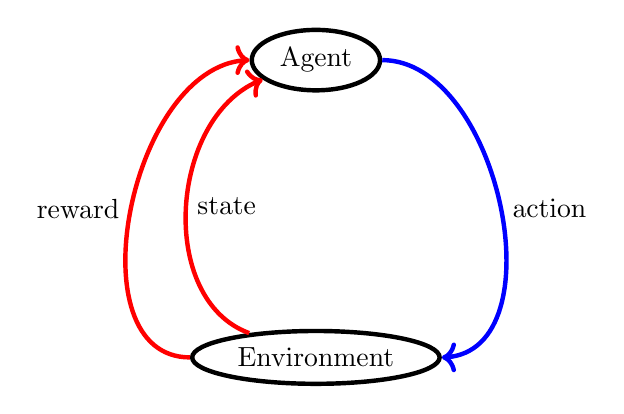
\begin{tikzpicture}

        \node[align=center, ellipse, draw, ultra thick] (a)  {Agent};
        \node[align=center, ellipse, draw, below=3cm of a, ultra thick] (e) {Environment};


        \draw[->, ultra thick, blue] (a) to[out=0, in=0] node [midway,
            right, text=black] {action} (e);
        \draw[->, ultra thick, red] (e) to[out=160, in=200]
            node [midway, right, text=black] {state} (a) ;
        \draw[->, ultra thick, red] (e) to[out=180, in=180]
            node [midway, left, text=black] {reward} (a);

    \end{tikzpicture}
    \caption{Reinforcement learning scenario \label{fig: 1}}
\end{figure}

At each step the agent faces a decision to choose an action leading to a new
state and the reward associated with it. Thereby the agent faces a dilemma in
this choice based on the previous experience with the state and action,
should the agent choose to export this information about the environment \&
states and optimize for the reward or should the agent explore other unknown
states potentially leading to a more favorable outcome. In reinforcement
learning this is called "exploration versus exploitation trade off.

Also, a key difference to traditional supervised learning, reinforcement
learning does not sample features based on a fixed distribution. Essentially
the training and testing phases are not separated, but rather combined in
each step.
\newline

The two main learning settings are distinguished, the setting where the
full environmental model is known and unknown.

The mathematical model which describes the agent's iteration with the
environment is the Markov decision process (MPD).
\begin{definition}[Markov decision process]
    The MDP is defined by 4 tuple $(S, A, \delta, R_a)$:
    \begin{itemize}
        \item The set of all states $S$, with a start state $s_0 \in S$,
        \item The set of all actions $A$,
        \item The transition probability $\mathbb{P}[s'|s, a] = \int_{S'}
            P_a(s, s') ds'$
        \item The reward probability $\mathbb{P}[r'|s, a] =
            \int_{S'}R_a\left(s', s  \right)ds' $
    \end{itemize}
\end{definition}
The transition probability $\mathbb{P}[s'|s, a]$ describes the probability of
the agent landing in state $s'$, when he is initially at state $s$ and takes
an action $a$. Similarity the reward probability is explained in the same way. The
structure of this state transition only depends on the last state and the
action taken and not on the whole history of states and actions hence the
Markov property and the naming of the model. Usually the state transitions and
rewards are deterministic, in this case the transition and reward probability
is $1$ and the MDP is called \textbf{deterministic} and the reward is $r(s, a)$.
\begin{figure}[ht!]
    \centering
    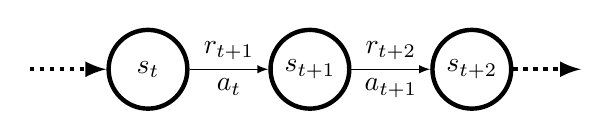
\begin{tikzpicture}

        \node[align=center, circle, draw, ultra thick, minimum size=1cm] (1)  {$s_t$};
        \node[align=center, circle, draw, ultra thick, right=of 1, minimum size=1cm] (2)
            {$s_{t+1}$};
        \node[align=center, circle, draw, ultra thick, right=of 2, minimum
            size=1cm] (3)
            {$s_{t+2}$};

        \draw[->, dotted, ultra thick, -latex] (-1.5, 0) to (1);
        \draw[->, dotted, ultra thick, -latex] (3) to (5.5, 0);
        \draw[->, -latex] (1) to node[midway, below] {$a_t$} node[midway,
            above] {$r_{t+1}$} (2);
        \draw[->, -latex] (2) to node[midway, below] {$a_{t+1}$} node[midway,
            above] {$r_{t+2}$} (3);

    \end{tikzpicture}
    \caption{Deterministic discrete MDP \label{fig: 2} \cite{ml_foundations}}
    \label{}
\end{figure}
In the discrete model the agent will preform actions in a set of decision
epochs $t \in {0,\ldots,T}$ \ref{fig: 2}, this is the usual model adopted for a wide range
of problems. The MDP is called \textbf{finite} when both $S$ and $A$ are
finite sets. Furthermore, the MDP has a \textbf{finite time horizon} when $T$
is finite.
\newline

The goal for the agent in an MPD is to find a good policy for the decision.
The policy is a function, which given a state returns a probability
distribution over the possible actions from the given state. The choice is
then the action with the highest probability.
\begin{definition}[Policy]
    A policy is a mapping $\pi : S \to \Delta\left( A \right)$, where $S$ is
    the state space and $\Delta(A)$ is the set of probability distributions
    over A.
    \newline

    We call the policy deterministic if:
    \begin{align}
        \forall s \in S\;\; \exists !  a\in A:\quad \pi(s)(a) = 1
    \end{align}
    In this case we have $\text{im}(\pi) = A$, and we can say $\pi: S \to A$ with
    $\pi(s) = a$.
\end{definition}
With the definition of a policy, the aim of the agent can be expressed as
trying to find a policy that maximizes the total return. For a discrete
policy the total return is
\begin{align}
    &\sum_{t=0}^{T} r(s_t, \pi(s_t)) & \text{finite horizon}\\
    &\sum_{t=0}^{\infty}\gamma^{t} r(s_t, \pi(s_t)) & \text{infinite horizon}
\end{align}
where $r(s_t, \pi(s_t))$ is the reward function for the next state and
$\gamma \in [0, 1)$ a discount factor for future rewards.
\newline
To quantify what is the optimal policy, it is natural to define the value of the
policy at a given state.
\begin{definition}[Policy value]
    The value $V_\pi(s)$ of the policy $\pi$ at state $s \in S$ is defined as
    the expected value of the total reward over the policy distribution
    $\pi(s_t)$ of state $s_t \in S$ at epoch $t \le T$. For the finite horizon
    it is
    \begin{align}
        V_\pi(s) = \mathbb{E}_{a_t\sim\pi(s_t)}\left[\sum_{t=0}^{T}r(s_t,
        a_t) \Bigg| s_0 = s \right].
    \end{align}
    For the infinite horizon for $\gamma \in [0, 1)$
    \begin{align}
        V_\pi(s) =
        \mathbb{E}_{a_t\sim\pi(s_t)}\left[\sum_{t=0}^{\infty}\gamma^{t} r(s_t,
        a_t) \Bigg| s_0 = s \right].
    \end{align}
\end{definition}
Thereby the optimal policy can be defined in the following way
\begin{definition}[Optimal policy]
    The policy $\pi^{*}$ is called optimal if for any policy $\pi$ it
    holds that
    \begin{align}
        V_{\pi^{*}}(s) \ge V_\pi(s) \quad \forall s \in S.
    \end{align}
\end{definition}
Similarly to the policy value we can give the pair $(s, a)$ associated to a
policy $\pi$ a value, the so called state-action value
\begin{definition}[State-action value]
    The state-action value function $Q_\pi$ associated with a policy $\pi$ is
    defined on all pairs state-action pairs $(s, a) \in S \times A$
    \begin{align}
        Q_\pi(s, a) &= \mathbb{E}[r(s,a)]
        \mathbb{E}_{a_t\sim\pi(s_t)}\left[ \sum_{t=1}^{\infty}\gamma^{t}
            r(s_t, a_t)\Bigg |\; s_0 = s,\; a_0 = a \right] \\
        \nonumber
            &= \mathbb{E}\left[r(s,a) + \gamma V_\pi(s_1)\Big| \;s_0=s,\;
            a_0=a   \right].
    \end{align}
    Note that the expected value of the state-value function at $(s, a)$ over the policy
    distribution at state $s$ is the policy value at $s$, i.e.
    \begin{align}
        \mathbb{E}_{a\sim\pi(s)}\left[Q_\pi(s, a)\right] = V_\pi(s).
    \end{align}
\end{definition}
With the help of these definitions it can be shown that for any MDP there is
a deterministic optimal policy.
\begin{theorem}[Policy Improvement Theorem]
    For any two policies $\pi'$ and $\pi$, it holds that
    \begin{align}
         &\mathbb{E}_{a\sim\pi'(s)}\left[Q_\pi(s, a)\right]
        \ge \mathbb{E}_{a\sim\pi(s)}\left[Q_\pi(s, a)\right]  \quad \forall s \in S
        \\
         &\quad \implies  V_{\pi'}(s) \ge V_\pi (s) \quad
         \forall s \in S\nonumber.
    \end{align}
\end{theorem}
\begin{theorem}[Bellman's optimality condition]
    A policy $\pi$ is optimal if and only if for all state-action pairs
    $(s, a) \in S x A$ with $\pi(s)(a) > 0$ it holds that
    \begin{align}
        a \in \argmax_{a'\in A} Q_\pi(s, a').
    \end{align}
\end{theorem}
\begin{theorem}{Existence of optimal deterministic policy}
    Any finite MDP has an optimal deterministic policy.
\end{theorem}
Consider an optimal deterministic policy $\pi^{*}$ with its policy value and
state-action value functions $V^{*}$ and $Q^{*}$. The optimal policy for all
state is
\begin{align}
    \pi^{*}(s) = \argmax_{a \in A} Q^{*}(s,a).
\end{align}
Thus, the agent only needs to know the state-action value function $Q^{*}$ to
determine the optimal policy, and does not need to have information about the
transition and reward probabilities. Using the definition of the state-value
function for $Q^{*}$, $V^{*}(s) = Q^{*}(s, \pi^{*}(s))$ gives a system of
equations called \textit{Bellman equations}:
\begin{align}
    V^{*}(s) = \max_{a\in A} \left\{ \mathbb{E}[r(s, a)] + \gamma\sum_{s'\in S}
    \mathbb{P}[s'|s,a] V^{*}(s') \right\} \quad \forall s \in S.
\end{align}
\begin{theorem}[Bellman Equations]
    The policy value $V_\pi(s)$ of a policy $\pi$ at state $s$ for an MDP
    with infinite horizon is subjected to the following linear system of
    equations
    \begin{align}
        V^{*}(s) = \mathbb{E}_{a_1 \sim \pi(s)}[r(s, a_1)] + \gamma\sum_{s'\in S}
        \mathbb{P}[s'|s, \pi(s)] V^{*}(s') \quad \forall s \in S.
    \end{align}
\end{theorem}
We can rewrite the linear system
\begin{align}
    v = \gamma P v + r,
\end{align}
where
\begin{align}
    &p_{s, s'} = \mathbb{P}[s'|s, \pi(s)] \quad \forall s,s' \in S \quad
    \text{is the transition probability matrix,}\\
    &v_s = V_\pi(s) \quad \forall s \in S \quad \text{is the value vector and }\\
    &r_s = \mathbb{E}[r(s, \pi(s)] \quad \forall s \in S \quad \text{is the reward
    vector}.
\end{align}
For an MDP with finite horizon with a known probability matrix $P$ and a
known reward expectation $r$, linear algebra gives a unique solution for
the value vector by matrix inversion
\begin{align}
    v^{*} = (I - \gamma P)^{-1} R,
\end{align}
where $I$ is the appropriate identity matrix.
\newline

Proofs for the theorems can be found in \cite[Chapter~17]{ml_foundations}.
\section{Monte Carlo Tree Search}
MCTS is a search algorithm for decision processes like MDP. The algorithm
focuses on finding the most favorable course of action by uniformly expanding
the search tree at each step and applying random actions/decisions until
reaching a terminal state, this outcome is then communicated back to the
start (backpropagation). In the last decade MCTS has been combined
with learning based methods \cite{alphazero} to produce agents which can beat
humans in Chess, GO and other games.
\newline

On a basic level the fundamental concept of the algorithm is that the true
value of an action can be approximated by random simulation, which ultimately
adjusts the policy efficiently to derive a best-first strategy
\cite{mcts_survey}. One search iteration is done in four steps:
\newline

\textbf{1. Selection Phase:} Also called Tree-Traversal Phase, starts at the
root node state and walks down until reaching a leaf node state with a
selection policy. The leaf node state is one that is not yet fully expanded,
i.e. has unvisited children or is not a terminal state. The selection policy of
the walk is done through the confidence bound ($UCB1$), where the idea
is to weight out and balance the exploration vs exploitation. The next action
is chosen such that the next node has the biggest $UCB1$ value. The basic
$UCB1$ formula is
\begin{align}
    UCB1 = \frac{w_i}{n_i} + C \sqrt{\frac{\ln N_i}{n_i}},
\end{align}
where $w_i$ is the number of wins of the node, $n_i$ the number of visits of
the node, $N_i$ the number of visits of the parent node and $C\in R$ is a
constant, usually chosen to be $C = \sqrt{2}$
\newline

\textbf{2. Node Expansion Phase:} An extra node is added into the tree according
to the available actions, if the node state is not a terminal one.
\newline

\textbf{3. Simulation Phase}: Also called Roll-out state. A simulation/roll-out
is from the current node selecting actions randomly until a terminal node
state.
\newline

\textbf{4. Backpropagation Phase:} The result of the simulation is used to
update the information in the nodes traversed, such as the outcome/reward of
the terminal state at the end of the simulation and also the visit count of
the nodes.
\begin{figure}[htb!]
    \centering
    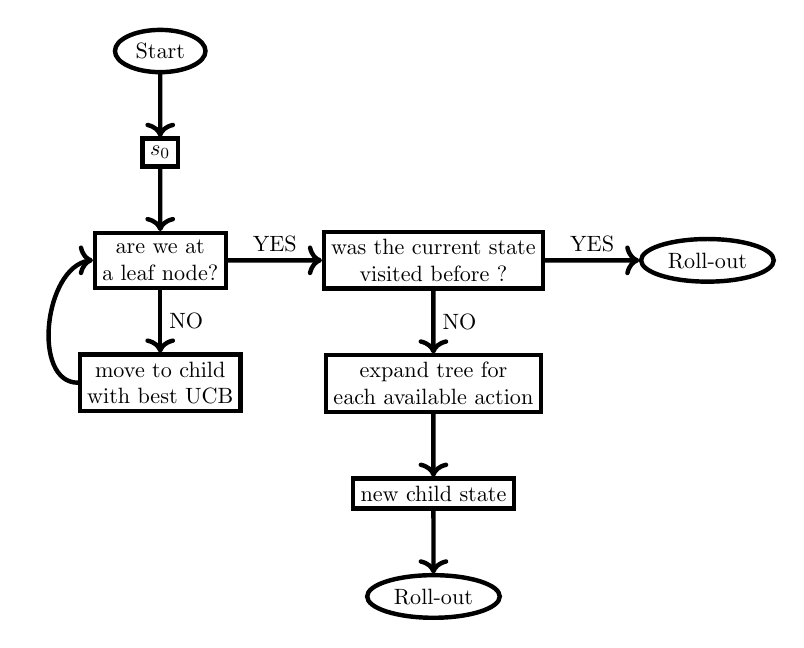
\begin{tikzpicture}[scale=0.8, transform shape]
        \node[align=center, ellipse, draw, ultra thick] (0)  {Start};

        \node[align=center, draw, ultra thick, below=of 0] (1)
            {$s_0$};

        \node[align=center, draw, ultra thick, below=of 1] (2)
            {are we at\\ a leaf node?};

        \node[align=center, draw, ultra thick, below=of 2] (3)
            {move to child\\ with best UCB};

        \node[align=center, draw, ultra thick, right=1.5cm of 2] (4)
            {was the current state\\ visited before ?};

        \node[align=center, ellipse, draw, ultra thick, right=1.5cm of 4] (5)
            {Roll-out};

        \node[align=center, draw, ultra thick, below=of 4] (6)
            {expand tree for\\each available action};

        \node[align=center, draw, ultra thick, below=of 6] (7)
            {new child state};

        \node[align=center,ellipse, draw, ultra thick, below=of 7] (8)
            {Roll-out};

        \draw[->, ultra thick] (0) to (1);
        \draw[->, ultra thick] (1) to (2);
        \draw[->, ultra thick] (2) to node[midway, right] {NO} (3);
        \draw[->, ultra thick] (2) to node[midway, above] {YES} (4);
        \draw[->, ultra thick] (4) to node[midway, above] {YES} (5);
        \draw[->, ultra thick] (4) to node[midway, right] {NO} (6);
        \draw[->, ultra thick] (6) to (7);
        \draw[->, ultra thick] (7) to (8);

        \draw[->, ultra thick, in=180, out=180] (3) to (2);

    \end{tikzpicture}
    \caption{MCTS algorithmic diagram \label{fig: 3}}
\end{figure}

The general algorithmic structure is described in \cite{mcts_survey}, denoted
in \ref{alg: 1}. For clarity purposes the diagram of the algorithm is in
\ref{fig: 3}.
\begin{algorithm}
\caption{MCTS Algorithm}\label{alg: 1}
    \begin{algorithmic}
        \Require state $s_0$
        \While{within computational budget}
            \State $s_k \gets \text{SelectionPolicy}(s_0)$
            \State  $w \gets \text{RollOut}(s_k)$
            \State $\text{BackPropagate}(s_k, w)$
        \EndWhile
        \Ensure $a\left(\text{BestChild}(s_0)\right)$
    \end{algorithmic}
\end{algorithm}
The search starts with an input state $s_0$, and selects the next set of
states based on the selection policy, which is are the states with the
biggest $UCB1$ value. The state $s_k$ is reached after the selection phase
and the expansion, upon which a simulation is run giving the terminal
result/outcome $w$. The outcome is then communicated back from $s_k$ back to the
root node in the path taken to reach $s_k$ from the root node. At the end the
algorithm returns then the  action $a$ leading to the best child of $s_0$.
The number of search iterations is usually indicated by a specific search
time or number of search steps given and is denoted by the while statement.

\section{Graph Neural Networks \label{sec: gnn}}
This section is an introductory the Graph Neural Networks (GNNs)
\cite{gnn_overview}. GNNs are Neural Networks (NNs) which operate over graph
structured data. Let further denote a graph as a tuple $(E, V)$, where $E$
are edges and $V$ are the nodes of the graph. Also let $A$ be the adjacency
matrix of the graph, where $a_{ij} = 1$ if $(i, j) \in E$ and $a_{ij} =0$
otherwise. Finally, denote $X$ to be the node features.
\newline

There are multiple types of GNNs some more complex than others
\cite{gnn_overview}, but the core principles are taken from convolutional
NNs. An image can be seen as a grid graph, where each node corresponds to a
pixel and is connected to its neighboring pixels. Simple convolution in
images aggregates pixel by applying a simple operation (kernel) on its
neighborhood, updating the pixels value. Similarly, in a graph the
convolutional GNN will take the information of the neighboring node features
(and edge features) to update the underlying node by applying some function
on them \ref{fig: 4}.
\begin{figure}[htb!]
    \centering
    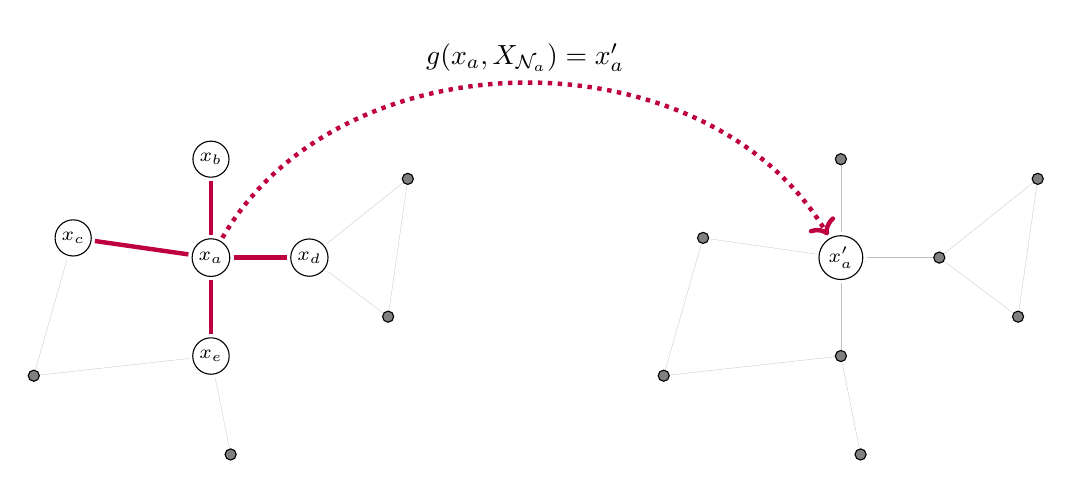
\begin{tikzpicture}
            \node [style=new style 0] (6) at (3.25, 1) {};
            \node [style=new style 0] (7) at (3, -0.75) {};
            \node [style=new style 0] (8) at (1, -2.5) {};
            \node [style=new style 0] (11) at (-1.5, -1.5) {};
            \node [style=1] (12) at (0.75, 0) {$x_a$};
            \node [style=1] (13) at (-1, 0.25) {$x_c$};
            \node [style=1] (14) at (0.75, 1.25) {$x_b$};
            \node [style=1] (15) at (2, 0) {$x_d$};
            \node [style=1] (16) at (0.75, -1.25) {$x_e$};

            \draw [style=new edge style 0] (6) to (7);
            \draw [style=new edge style 0] (15) to (7);
            \draw [style=new edge style 0] (15) to (6);
            \draw [style=new edge style 0] (16) to (8);
            \draw [style=new edge style 0] (11) to (16);
            \draw [style=new edge style 0] (13) to (11);
            \draw [style=new edge style 1] (12) to (16);
            \draw [style=new edge style 1] (12) to (15);
            \draw [style=new edge style 1] (13) to (12);
            \draw [style=new edge style 1] (14) to (12);



            \node [style=new style 0] (21) at (11.25, 1) {};
            \node [style=new style 0] (22) at (11, -0.75) {};
            \node [style=new style 0] (23) at (9, -2.5) {};
            \node [style=new style 0] (24) at (6.5, -1.5) {};
            \node [style=1] (17) at (8.75, 0) {$x_a'$};
            \node [style=new style 0] (25) at (7, 0.25) {};
            \node [style=new style 0] (26) at (8.75, 1.25) {};
            \node [style=new style 0] (27) at (10, 0) {};
            \node [style=new style 0] (28) at (8.75, -1.25) {};

            \draw [style=new edge style 0] (26) to (17);
            \draw [style=new edge style 0] (17) to (25);
            \draw [style=new edge style 0] (17) to (27);
            \draw [style=new edge style 0] (17) to (28);
            \draw [style=new edge style 0] (28) to (24);
            \draw [style=new edge style 0] (28) to (23);
            \draw [style=new edge style 0] (27) to (21);
            \draw [style=new edge style 0] (27) to (22);
            \draw [style=new edge style 0] (21) to (22);
            \draw [style=new edge style 0] (25) to (24);

            \draw [style=new edge style 1, in=120, out=60, dotted, ->] (12)
                to node[midway, above] {$g(x_a, X_{\mathcal{N}_a}) = x_a'$} (17);
    \end{tikzpicture}
    \caption{Convolutional GNNs: simple example \label{fig: 4}}
\end{figure}

For a graph we can define a node's neighborhood, for a node $i \in V$ a
nodes 1-hop neighborhood is
\begin{align}
    \mathcal{N}_i := \left\{ j: (i,j) \in E\; \wedge \; (j, i) \in E
    \right\}.
\end{align}
The features of the 1-hop neighborhood $\mathcal{N}_i$ of the node are
\begin{align}
    X_{\mathcal{N}_i} = \left\{ \left\{ x_j: j \in \mathcal{N}_i \right\}
    \right\} .
\end{align}
Then the convolutional function $g$ operates on the features of the node
itself and on the features of its 1-hop neighborhood $g\left(x_i,
X_{\mathcal{N}_i}\right)$. Suitable functions that preserve the invariance
or equivariance of the graph. When applying a permutation matrix $P$ we need
to permute the rows and the columns of the adjacency matrix $A$, which
results to $PAP^{T}$, leading to functions satisfying
\begin{align}
    &f(PX, PAP^{T}) = f(X, A) \quad \text{Invariance}\\
    &f(PX, PAP^{T}) = Pf(X, A) \quad \text{Equivariance}
\end{align}
By applying the local function $g$ on all nodes and their neighborhoods we
get
\begin{align}
    f(X, A) =
    \begin{bmatrix}
        g(x_1, X_{\mathcal{N}_1})\\
        \vdots\\
        g(x_n, X_{\mathcal{N}_n})
    \end{bmatrix},
\end{align}
thus $g$ needs to be permutation invariant, to not depend on the order in
$X_{\mathcal{N}_i}$ and thereby $f$ will be equivariant. Conventionally the
local function $g$ is referred to as "`diffusion"' , "`propagation"' or
"`message passing"'
and the global function $f$ as a "`GNN Layer"' \cite[Chapter~5]{gnn_overview}.
The majority of the GNN Layer types can be
differentiated by three types, \textit{Convolutional}, \textit{Attentional}
and \textit{Message-passing} GNN. They are all different in the sense how $g$
incorporates the neighboring features, where $g$ needs to be permutation
invariant.
\newline

The convolutional type \cite[Chapter~5]{gnn_overview} as described above for
clarification, the features of the neighbors are aggregated additionally with
fixed weights $c_{ij}$ after applying some function $\psi$ on them
\begin{align}
    x_i' = g\left( x_i, \bigoplus_{j\in \mathcal{N}_i} c_{ij} \psi(x_j) \right).
\end{align}

In attention type \cite{gan_velickovic} features of neighbors are applied
with implicit weights, via attention. The attention coefficient for each
pair is computed via a function $\alpha_{ij} = a(x_i, x_j)$, usually a
softmax function resulting in
\begin{align}
    x_i' = g\left( x_i, \bigoplus_{j\in \mathcal{N}_i} a(x_i, x_j) \psi(x_j) \right).
\end{align}

The message passing type \cite[Chapter~5]{gnn_overview} computes arbitrary
vector "`messages"', these are then sent through the edges back to the
original node which gives
\begin{align}
    x_i' = g\left( x_i, \bigoplus_{j\in \mathcal{N}_i} \psi(x_i, x_j) \right).
\end{align}

In practice the functions $g$ and $\psi$ are learnable and are represented by
some appropriate NN structure and the $\bigoplus$ operator is a nonparametric
operation e.g. sum, mean, maximum or a recurrent neural network
\cite[Chapter~5]{gnn_overview}.
\newline

Dealing with real world networks it is piratical to incorporate edge
attributes in the GNN mechanism. For the attention type this is done with
success in the original paper GAT \cite{gan_velickovic} and improved on in
\cite{wsgat} by allowing signed weights through the attention coefficient.
The computation of the attention coefficient is the following
\begin{align}
    \alpha_{ij}^{(k)} = \text{sign}\left(e_{ij}  \right) \cdot
    \text{softmax}_j\left(\text{abs}(e_{ij}^{(k)})\right),
\end{align}
where
\begin{align}
    e_{ij}^{(k)} = \text{MLP}^{k}\left(h_i^{(k)} \| h_j^{(k)} \| w_{ij}\right).
\end{align}
Here $\|$ is the concatenation operator,  $w_{ij}$ is the weight
of the edge, $\text{MLP}^{k}$ is a $k$-th layer multilayer perceptron, where
the last weight can produce negative values, $h_i^{(k)}$ and $h_j^{(k)}$ is
the node feature embeddings after the $k$-th GNN layer. The input features
are in the 0-th layer $h_i^{(0)} = x_i$. Then the node embedding for the next
layer is calculated by
\begin{align}
    h_{i}^{(k+1)} = g\left( h_i^{(k)},
    \bigoplus_{j\in\mathcal{N}_i}\alpha_{ij}^{(k)}h_j^{(k)} \right)
\end{align}
\section{AlphaZero}
The section is a brief overview of how AlphaZero \cite{alphazero} works. The
special thing about AlphaZero is that it uses purely reinforcement learning
to optimize the policy and there is are is no outside data fed in. There are
two separate phases for making the model work with purely
reinforcement learning, in the one phase the model plays with itself and
gathers information about the environment and gathers the data. In the second
phase the information of the self play part is used to optimize the model and
then AlphaZero plays with the optimized model against itself again, forming a
loop \ref{fig: 5}.
\begin{figure}[htb!]
    \centering
    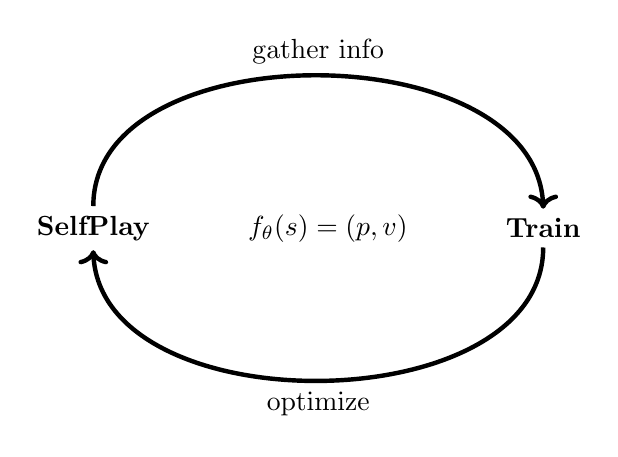
\begin{tikzpicture}
        \node[font=\bfseries] (0) {SelfPlay};
        \node[right=of 0] (1) {$f_{\theta}(s) = (p, v)$};
        \node[font=\bfseries, right= of 1] (2) {Train};

        \draw[->, ultra thick] (0) to[out=90, in=90] node[midway, above]
            {gather info} (2);
        \draw[->, ultra thick] (2) to[out=270, in=270] node[midway, below]
            {optimize} (0);
    \end{tikzpicture}
    \caption{AlphaZero cycle \label{fig: 5}}
\end{figure}
The optimization is done through the parameters $\theta$ of a deep neural
network $f_\theta(s) = (p, v)$, which takes a state as input and outputs the
transition probability vector $p_a = \mathbb{P}[a|s]$ for each action and a
scalar value $v$, which estimates the outcome of position $s$, $v \simeq
\mathbb{E}[r|s]$.
In the self-play phase the model uses the MCTS algorithm to traverse down the
MDP tree from the root node $s_0$. The key difference in the walk to a leaf
node is that alpha zero incorporate the output of $f_\theta(s)$ in $UCB$
formula, which can be expressed as follows
\begin{align}
    UCB = Q(s,a) + U(s,a),
\end{align}
where $Q(s,a)$ is the state-action value, and $U(s,a)\propto
\frac{P(s,a)}{1+N(s,a)}$ a value dependent on the node visit count $N(s, a)$
and probability $P(s, a)$ given by the deep neural network $f_\theta(s)$.
Furthermore, AlphaZero does not utilize the third phase of the MCTS algorithm
which randomly applies actions until reaching a terminal state. Instead, it
just proceeds with the fourth phase of MCTS, of evaluating the current state
and backpropagating to the root state. The architecture of $f_\theta$ is
highly dependent on game/problem learned. Generally the first thing is state
encoding, that is encoding the state in a usable way in AlphaGo
Zero\cite{alphazero} the state is encoded in a $19x19x17$ array, instead of a
simple $19x19$ board. The encoded state is passed residual neural network
where the output is split into a value head neural network with zero-centered
activation function to produce $v$ and a policy head neural network with
softmax activation function to output $p$.
[TODO: mb picture here for the architecture]

\section{Application to Problem}
The problem finding a path starting and ending at the same node with no
repeated edges which minimizes the weights is an NP-hard because it is a case
of a traveling salesman problem (TSV). As a first exploration step AlphaZero
is applied on the problem. The underlying MDP is a deterministic one, since
taking an action corresponds using an edge to get to the next node. The MDP
has also with finite horizon, dependent on the graph size. The agent starts
at a node $v_0$ corresponding, follows a policy to take actions/edges leading
to the next node $v_1$ until forming a circuit $\left\{ v_0, v_1, \ldots, v_0
\right\}$. The valid actions are edges from the current node $v_i$ that have
not yet been traversed. The state could be the path the agent is currently
taking, i.e. a sequence of nodes $s = \left\{ v_0,v_1,\ldots \right\}$. Upon
arrival of the terminal state, which is either a circuit or a dead end the
reward $R$ must be assigned correspondingly. It makes sence to keep a track
of the agents "`score"', such that the model will try to find the path with the
highest score. The score should be higher based on the sum of the weights and
the number of actions taken. . The agent should be punished with a negative
reward upon ending up at a terminal state which is not the desired circuit,
i.e. dead end. So the total reward will be combined from a global reward
(winning or losing) and a local reward (weight minimization/score)
\newline

Steps have been taken in implementing the problem in python and applying the
MCTS algorithm on the problem. The current difficulties aeries when trying to
implement AlphaZero because of the state encoding. The state encoding in
graph based problems needs to be done through GNNs, but the output also needs
to consider valid moves which are the edges not traversed. Hence, it might
make sense to somehow encode the valid moves in the input through dynamic
edges, i.e. removing edges. This is implemented in \cite{rl_coopt} by
masking, and with encoder-decoder layer. But will the removal of the edges
even make, since from a reinforcement learning perspective ? How should the
input layer look like ? The code can be found in \cite{github}.
\newline

To construct the encoded input it is useful to pass information about the
weights, edges visits, node/edge embeddings and current node/state. For the
weights, a weighted adjacency matrix of the graph can be used. For the edge
visits a binary matrix of the size of the adjacency matrix can be used, where
$1$ indicates the edge as visited and $0$ as unvisited. And the node/edge
embeddings a variation of methods described in section \ref{sec: gnn} can be
used. Lastly, as an indicator for the current node position the agent is in.
Similarly like in AlphaGo Zero, the information of the previous couple of
states can be concatenated together to get a promising input.


\input{./chapters/chapter4.tex}

\nocite{*}
\printbibliography

\end{document}
